\documentclass[aspectratio=1610]{beamer}

\usepackage{amsmath}
\usepackage{multirow}
\usepackage{hyperref}
\usepackage{booktabs}
\usepackage{tabularx}
\usepackage{graphicx}

\usepackage{listings}
\lstloadlanguages{C++,Java}
\lstset{language=Java,tabsize=2,aboveskip=-22pt,belowskip=-22pt}

\pdfpagebox5

\newcounter{exCnt}

\newcommand{\Emph}[1]{
  \textcolor{blue}{#1}
  }

\graphicspath{{./figs}}

% usage \fig{000} inserts PNG with name ending in 000 from figs folder, scale 1
%   \fig[0.5]{000} same file from figs folder but scaled with a 0.5 factor
\newcommand{\fig}[2][1]{
  \includegraphics[scale=#1]{n4l1-#2.png}
  }


\begin{document}

\begin{frame}[plain]
\begin{beamercolorbox}[rounded=true,shadow=true]{titlelike}
{\LARGE
\begin{center}
  CPSC 3780: Labs N4 and Lab1
\end{center}
}
\end{beamercolorbox}
\vfill
\parbox{.45\textwidth}{Oct 15, 2024
}
\end{frame}


%%%%%%%%%

\begin{frame}[plain,t]{Agenda}

  Objective: get started on Assignments A3 (individual) and PA4 (team).
  \begin{itemize}
  \item Set up a project team.
  \item 50 min: LAB N4, implementing sliding window functions.
  \item 50 min: LAB 1, starting a VM in Kathara, connected to the host machine.
  \end{itemize}

  Continue working on the labs after the class...
  
\end{frame}

%%%%%%%%

\begin{frame}[plain,t]{Project team selection}

  Load the Moodle course page. Go to Project and lab / Choose project teams:

  \vfill
  \fig[0.3]{000}  
  \vfill
\end{frame}

%%%%%%%%

\begin{frame}[plain,t,fragile]{N4: sliding windows (50 min)}

  \textbf{Work with your project team.} We want classes that manage sequence numbers only!

  Can you think of a generic \Emph{sliding window} class:
  \begin{enumerate}
  \item Start with a simple counter $\mod 2^b$

\begin{verbatim}
  SetMod(8); Add() -> 0; Add() -> 1; ... Add() -> 7; Add() -> 0; ...
\end{verbatim}

\item Define a window of size $w$; add to one end, remove from the other end:

\begin{verbatim}
  SetMod(8); SetWindow(3); Add():[0]; Add():[0,1]; Get()->0, [1];
  Add(): [1,2]; Add(): [1,2,3]; Add(): [1,2,3] window full;
  Get()->1, [2,3]; ... 
\end{verbatim}

\item Complete the activities from N4. Can you implement the functions using the generic sliding window class above?
  \end{enumerate}
\end{frame}


  %%%%%%%

\begin{frame}[plain,t]{L1: kathara vstart --bridged (50 min)}

  Start Lab 1 (Chapter 12). By the end of the lab, students will gain some familiarity with Kathara, and will understand the following general concepts:

  \begin{columns}
\column{.5\linewidth}
    \begin{itemize}
    \item The difference between the host machine and the virtual machine.
    \item One can access files on the host machine from the virtual machine.
    \item Computer network $\leftrightarrow$ Graph.
    \item Machine $\leftrightarrow$ Node in the graph.
    \item Network interface card (NIC) from machine $\leftrightarrow$ Arc incident to the node.
    \item Network cards are assigned \emph{network addresses}
    \item A machine can have as many network addresses as NICs.
    \end{itemize}

    \column{.5\linewidth}
    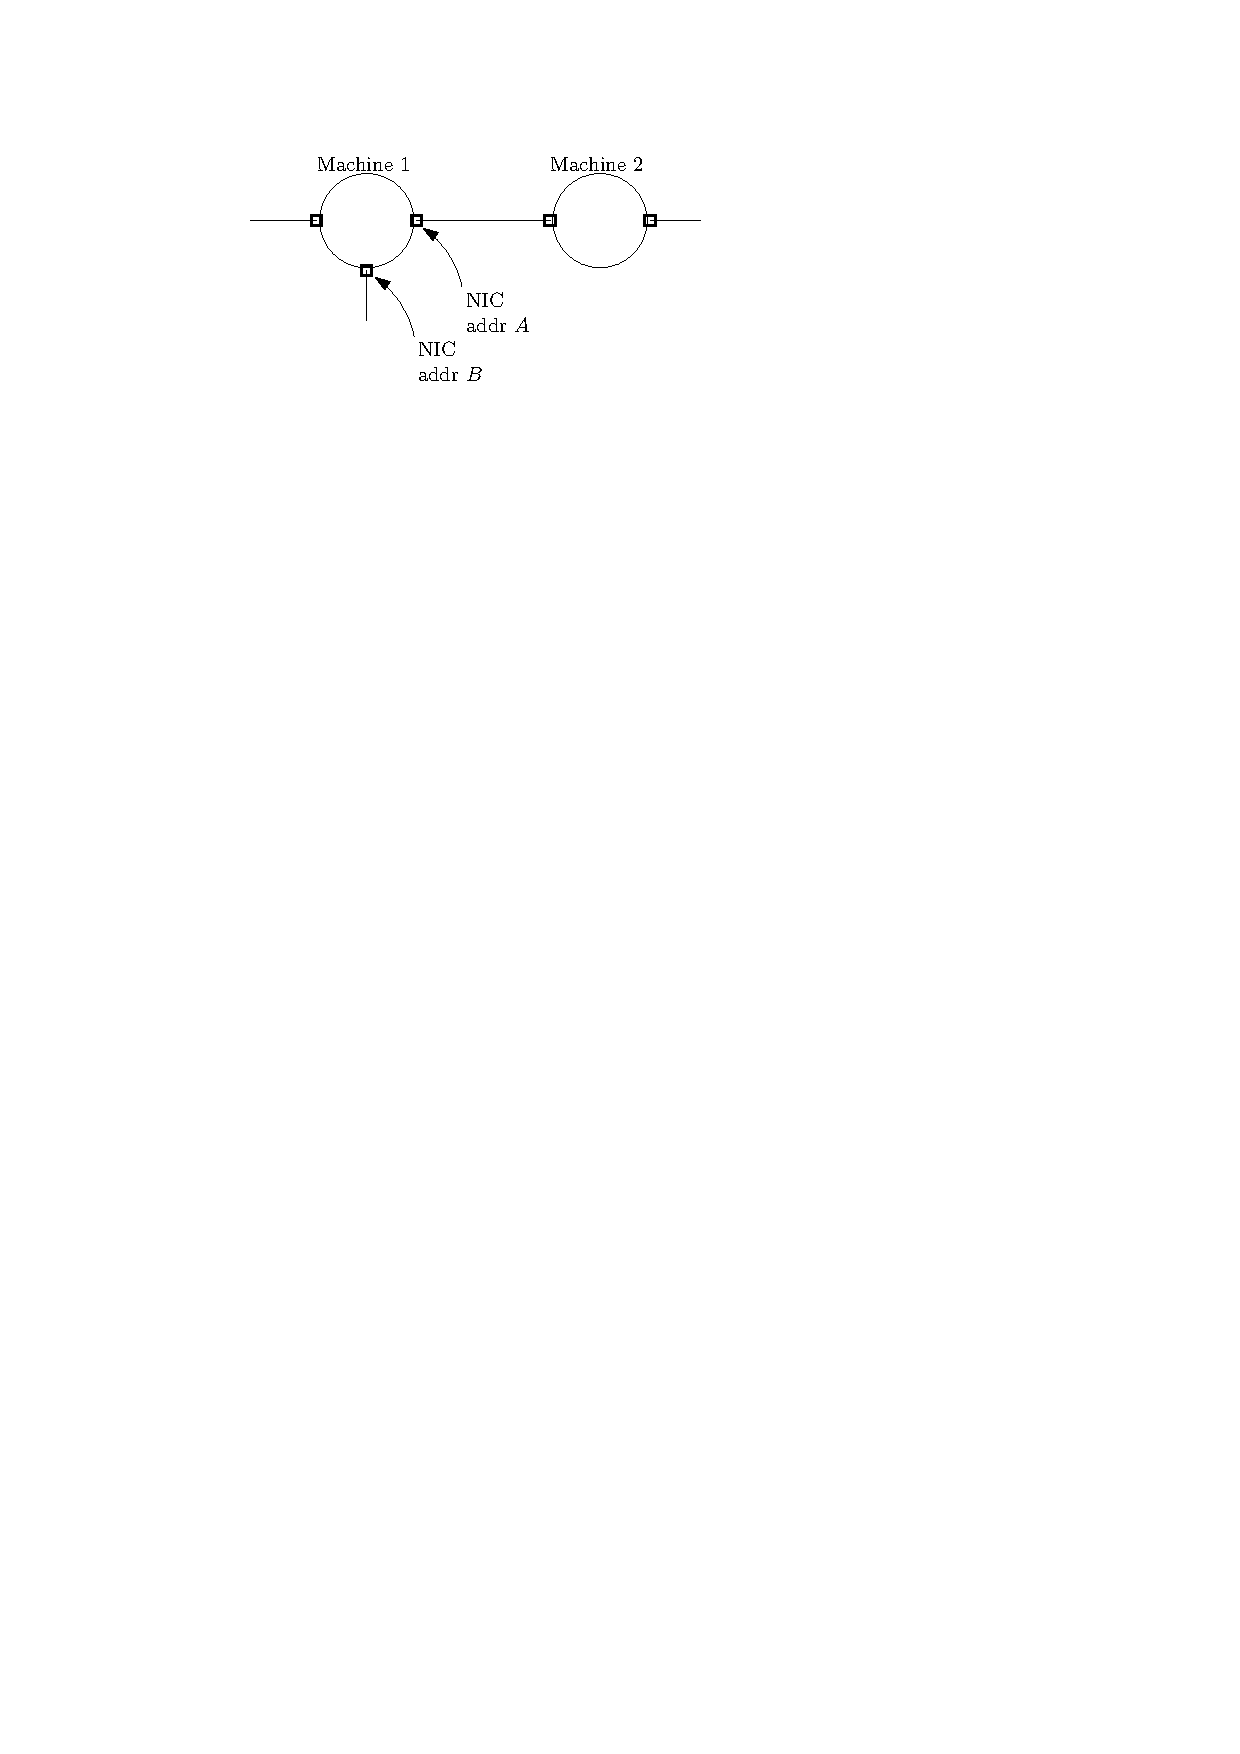
\includegraphics[page=1,scale=0.7]{n4l1-001.pdf}
  \end{columns}
\end{frame}
  
\end{document}
